\documentclass[compress]{beamer}
% !TeX document-id = {f19fb972-db1f-447e-9d78-531139c30778}
% !BIB program = biber

%\documentclass[handout]{beamer}
%\documentclass[compress]{beamer}
\usepackage[T1]{fontenc}
\usetheme[block=fill,subsectionpage=progressbar,sectionpage=progressbar]{metropolis} 
\usepackage{graphicx}

\usepackage{wasysym}
\usepackage{etoolbox}
\usepackage[utf8]{inputenc}

\usepackage{pifont}

\usepackage{threeparttable}
\usepackage{subcaption}

\usepackage{tikz-qtree}
\usepackage{neuralnetwork}

\setbeamercovered{still covered={\opaqueness<1->{5}},again covered={\opaqueness<1->{100}}}


\usepackage{listings}

\lstset{
	basicstyle=\scriptsize\ttfamily,
	columns=flexible,
	breaklines=true,
	numbers=left,
	%stepsize=1,
	numberstyle=\tiny,
	backgroundcolor=\color[rgb]{0.85,0.90,1}
}



\lstnewenvironment{lstlistingoutput}{\lstset{basicstyle=\footnotesize\ttfamily,
		columns=flexible,
		breaklines=true,
		numbers=left,
		%stepsize=1,
		numberstyle=\tiny,
		backgroundcolor=\color[rgb]{.7,.7,.7}}}{}


\lstnewenvironment{lstlistingoutputtiny}{\lstset{basicstyle=\tiny\ttfamily,
		columns=flexible,
		breaklines=true,
		numbers=left,
		%stepsize=1,
		numberstyle=\tiny,
		backgroundcolor=\color[rgb]{.7,.7,.7}}}{}


% color-coded listings; replace those above 
\usepackage{xcolor}
\usepackage{minted}
\definecolor{listingbg}{rgb}{0.87,0.93,1}
\setminted[python]{
	frame=none,
	framesep=1mm,
	baselinestretch=1,
	bgcolor=listingbg,
	fontsize=\scriptsize,
	linenos,
	breaklines
	}


\usepackage[american]{babel}
\usepackage{csquotes}
\usepackage[style=apa, backend = biber]{biblatex}
\renewcommand*{\bibfont}{\tiny}


\usepackage{tikz}
\usetikzlibrary{shapes,arrows,matrix}
\usepackage{multicol}

\usepackage{subcaption}

\usepackage{booktabs}
\usepackage{graphicx}



\makeatletter
\setbeamertemplate{headline}{%
	\begin{beamercolorbox}[colsep=1.5pt]{upper separation line head}
	\end{beamercolorbox}
	\begin{beamercolorbox}{section in head/foot}
		\vskip2pt\insertnavigation{\paperwidth}\vskip2pt
	\end{beamercolorbox}%
	\begin{beamercolorbox}[colsep=1.5pt]{lower separation line head}
	\end{beamercolorbox}
}
\makeatother





\setbeamercolor{section in head/foot}{fg=normal text.bg, bg=structure.fg}


\newcommand{\instruction}[1]{\emph{\textcolor{gray}{[#1]}}}



\newcommand{\question}[1]{
	\begin{frame}[plain]
	\begin{columns}
		\column{.3\textwidth}
		\makebox[\columnwidth]{
			\includegraphics[width=\columnwidth,height=\paperheight,keepaspectratio]{mannetje.png}}
		\column{.7\textwidth}
		\large
		\textcolor{orange}{\textbf{\emph{#1}}}
	\end{columns}
\end{frame}}


\tikzstyle{block} = [rectangle, draw, fill=blue!20, 
text width=5em, text centered, rounded corners, minimum height=4em]
\tikzstyle{line} = [draw]
\tikzstyle{pijltje} = [draw, -latex']
\tikzstyle{cloud} = [draw, ellipse,fill=red!20, node distance=3cm,
minimum height=2em, text width=4em, text centered,]


\setbeamercovered{transparent}

\addbibresource{../../resources/literature.bib}
\graphicspath{{../../resources/img/}}


\begin{document}

\title[Big Data and Automated Content Analysis]{\textbf{Big Data and Automated Content Analysis (12EC)} 
\\Week 13: »Multimedia Data«
\\Wednesday}
\author[Felicia Loecherbach]{Felicia Loecherbach\\ \footnotesize{f.loecherbach@uva.nl \\}}
\date{May 10, 2023}
\institute[UvA CW]{UvA RM Communication Science}


\begin{frame}{}
	\titlepage
\end{frame}

\begin{frame}{Today}
	\tableofcontents
\end{frame}
%\begin{frame}[standout]
%Before we start: Questions from last week?
%\end{frame}


\begin{frame}[standout]
Today: Beyond words: Multimedia Data
\end{frame}





\section{Multimedia data}


\subsection{The shift towards multimedia data}

\begin{frame}{Why do Images Matter?}
  \large{People are more likely to pay attention to visuals}
  
  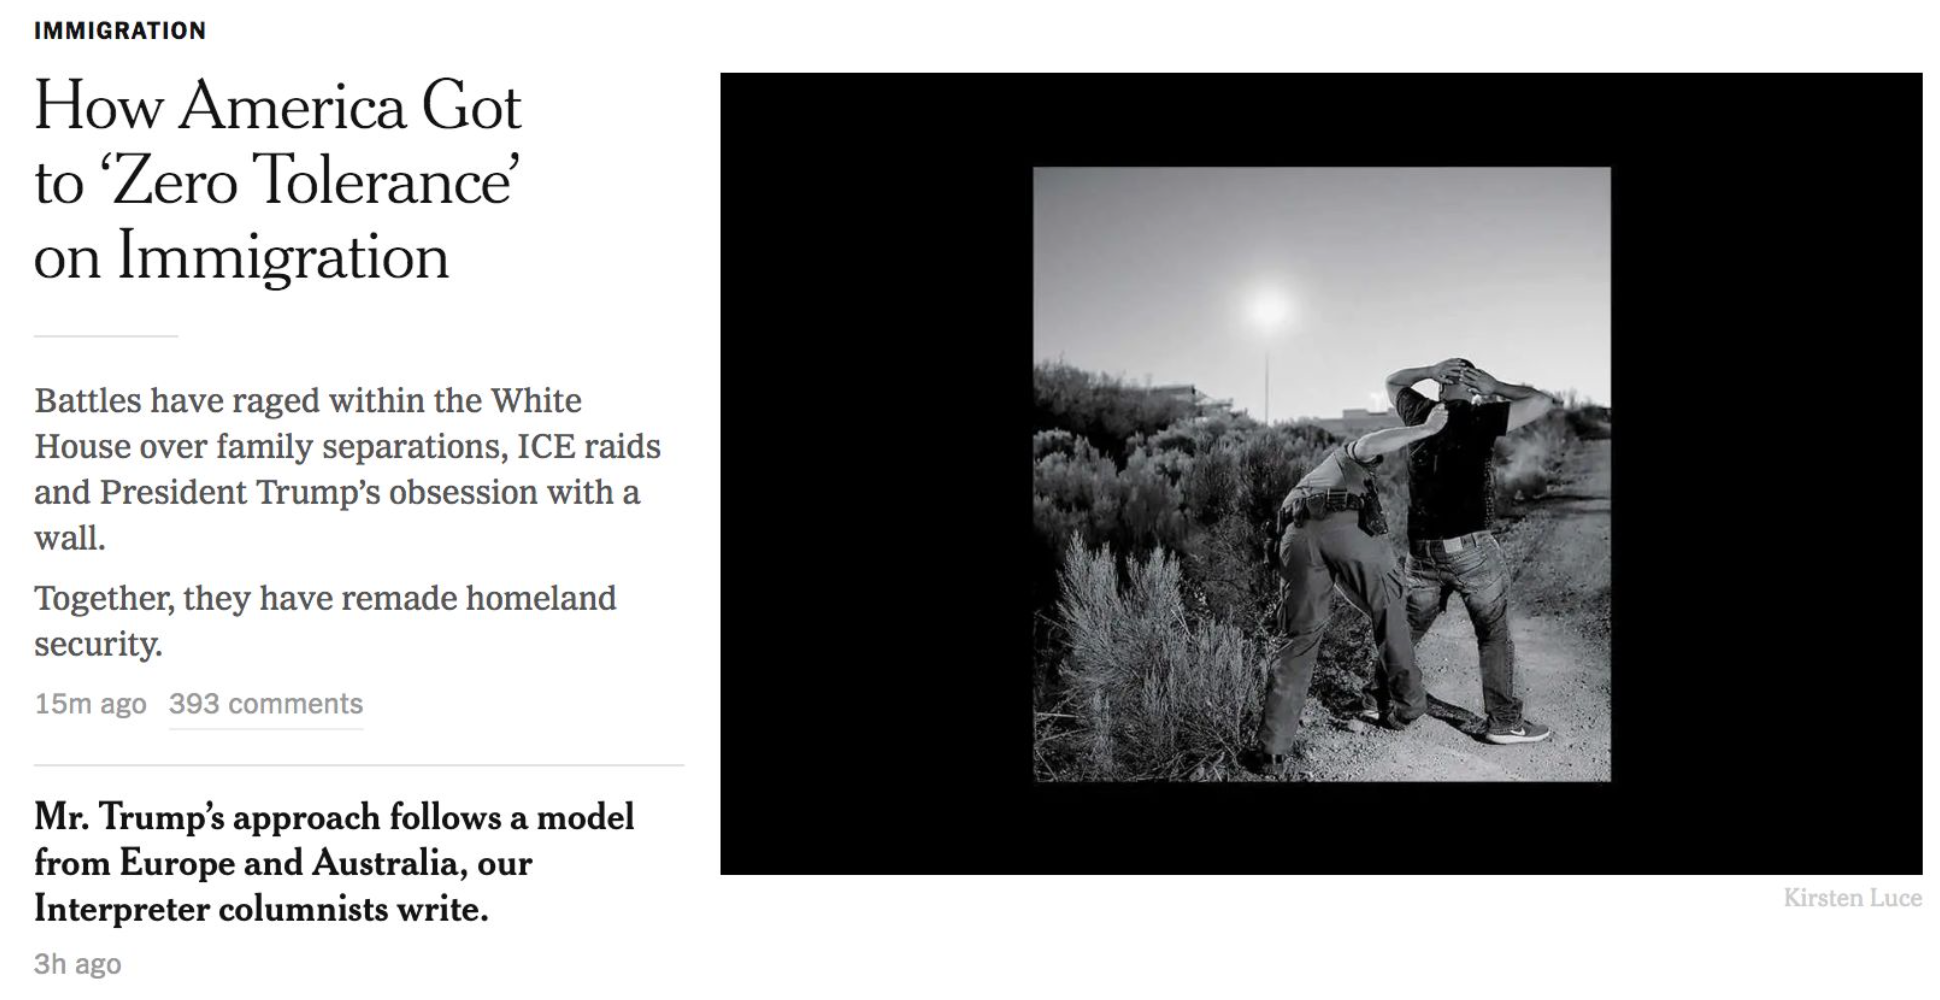
\includegraphics[scale=0.3]{framing-nyt.png} \centering
  
  \vfill
  \footnotesize Dahmen (2012) ``\textit{Photographic Framing in the Stem Cell Debate}''
  
  \end{frame}
  
  %%%%%%%%%%%%%%%%%%%%
  \begin{frame}{Why do Images Matter?}
  \large{People are more likely to recall information learned through visuals}
  
  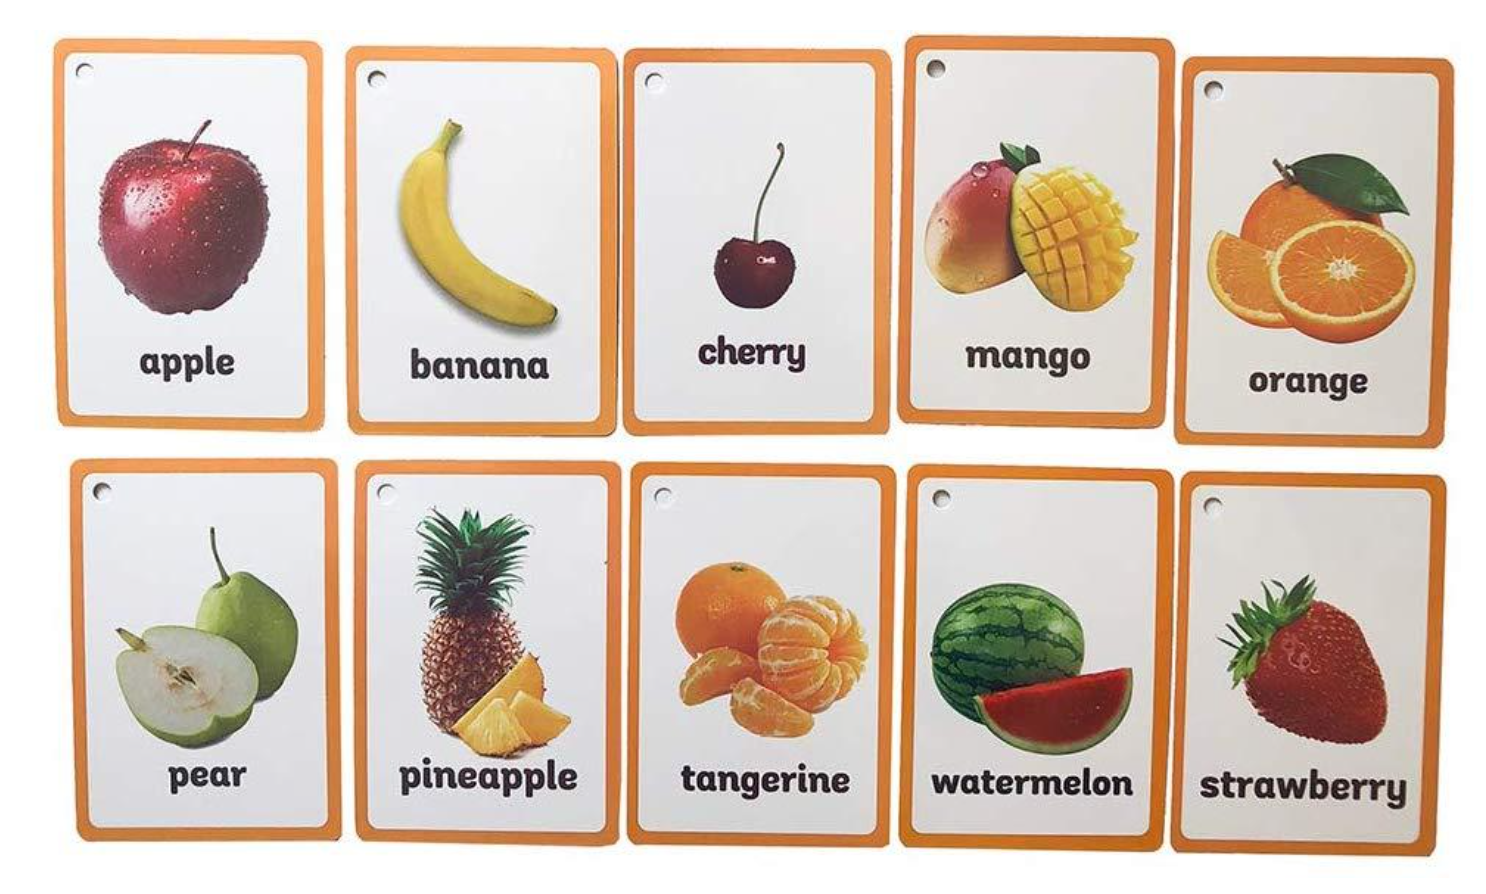
\includegraphics[scale=0.3]{recall.png} \centering
  
  \vfill
  \footnotesize Paivio et al. (1968) ``\textit{Why are pictures easier to recall than words?}''
  
  \end{frame}
  
  %%%%%%%%%%%%%%%%%%%%
  \begin{frame}{Why do Images Matter?}
  \large{Visuals evoke stronger emotional reactions}
  
  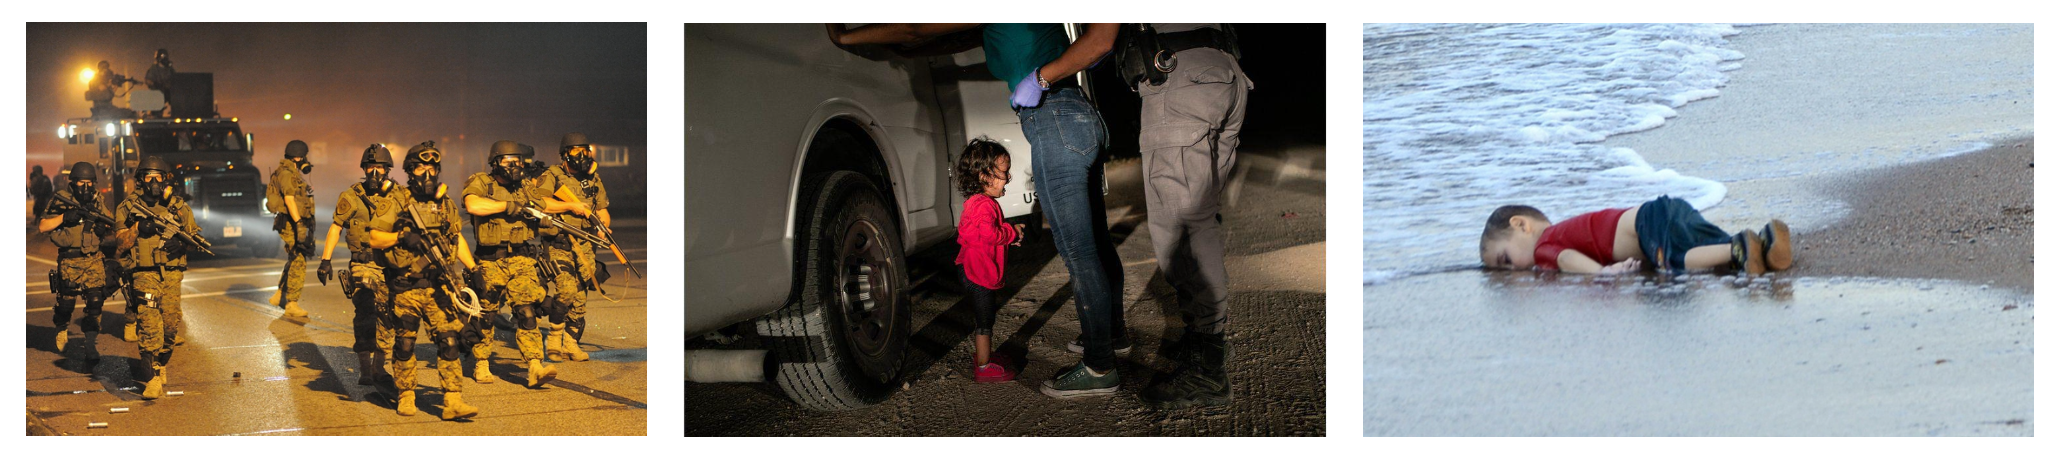
\includegraphics[scale=0.3]{emotions.png} \centering
  
  \vfill
  \footnotesize Grabe \& Bucy (2009) ``\textit{Images Bite Politics}''
  
  \end{frame}
  
  
  %%%%%%%%%%%%%%%%%%%%
  \begin{frame}{Why do Images Matter?}
  \large{Image effects in \textbf{politics}: images $\rightarrow$ inference of competence $\rightarrow$ voting}
  
  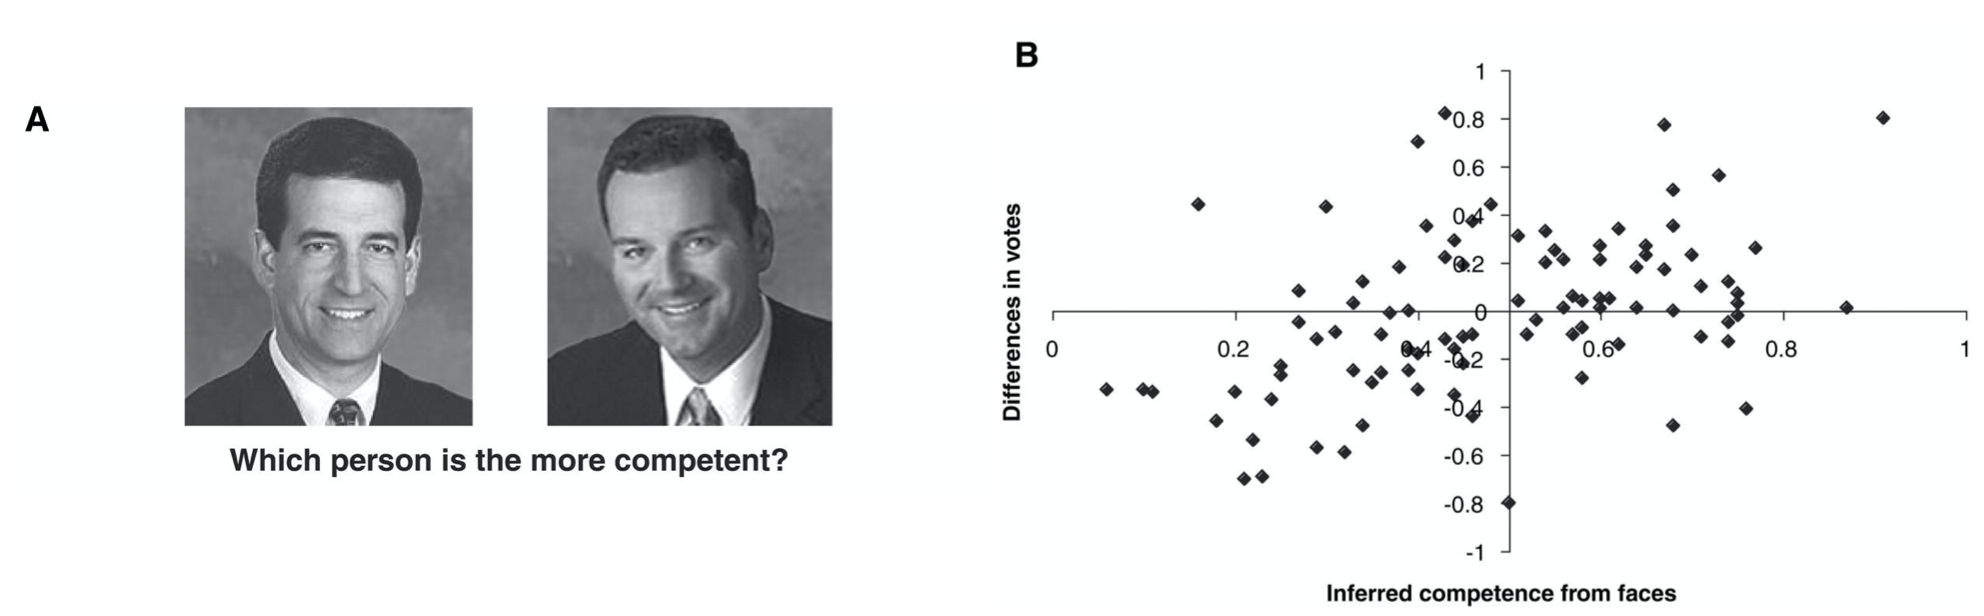
\includegraphics[scale=0.3]{todorov.png} \centering
  
  \vfill
  \footnotesize Todorov et al. (2009) ``\textit{Inferences of Competence from Faces Predict Election Outcomes}''
  
  \end{frame}
  
  %%%%%%%%%%%%%%%%%%%%
  \begin{frame}{Why do Images Matter?}
  \large{Image effects in \textbf{politics}: images $\rightarrow$ framing $\rightarrow$ attitudes}
  
  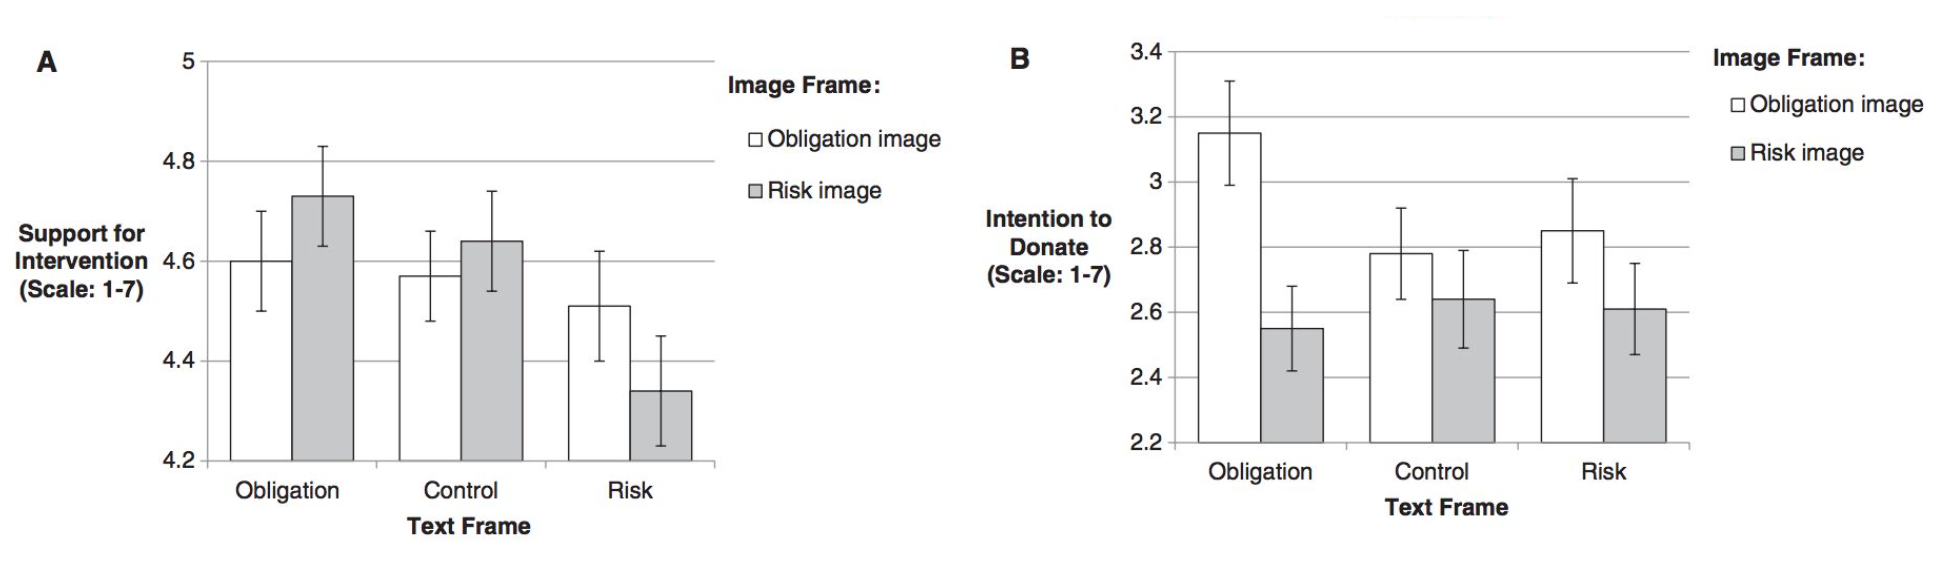
\includegraphics[scale=0.3]{framing_politics.png} \centering
  
  \vfill
  \footnotesize Powell et al. (2015) ``A Clearer Picture''
  
  \end{frame}
  
  
  %%%%%%%%%%%%%%%%%%%%
  \begin{frame}{Why do Images Matter?}
  \large{Image effects in \textbf{politics}: images $\rightarrow$ emotions $\rightarrow$ \textbf{mobilization}}
  
  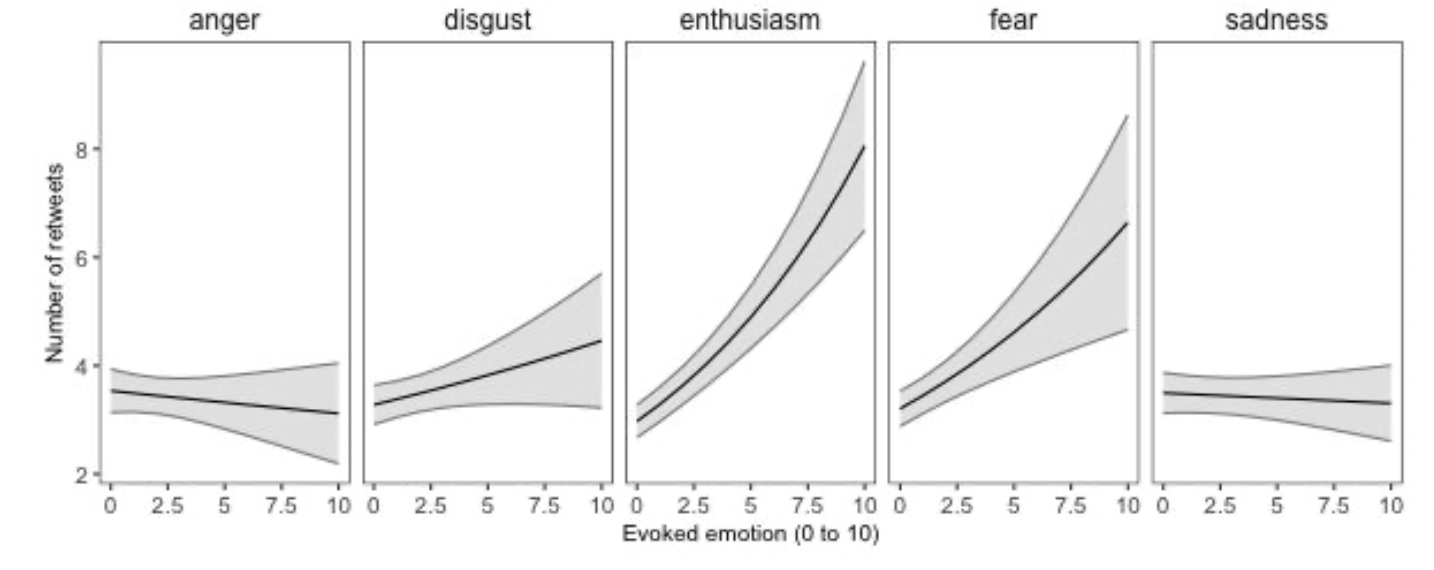
\includegraphics[scale=0.3]{casas_williams.png} \centering
  
  \vfill
  \footnotesize Casas \& Webb Williams (2018) ``Images That Matter''
  
  \end{frame}
  
  %%%%%%%%%%%%%%%%%%%%
  \begin{frame}{Why do Images Matter?}
  \large{Images are more central than even in our life}
  
  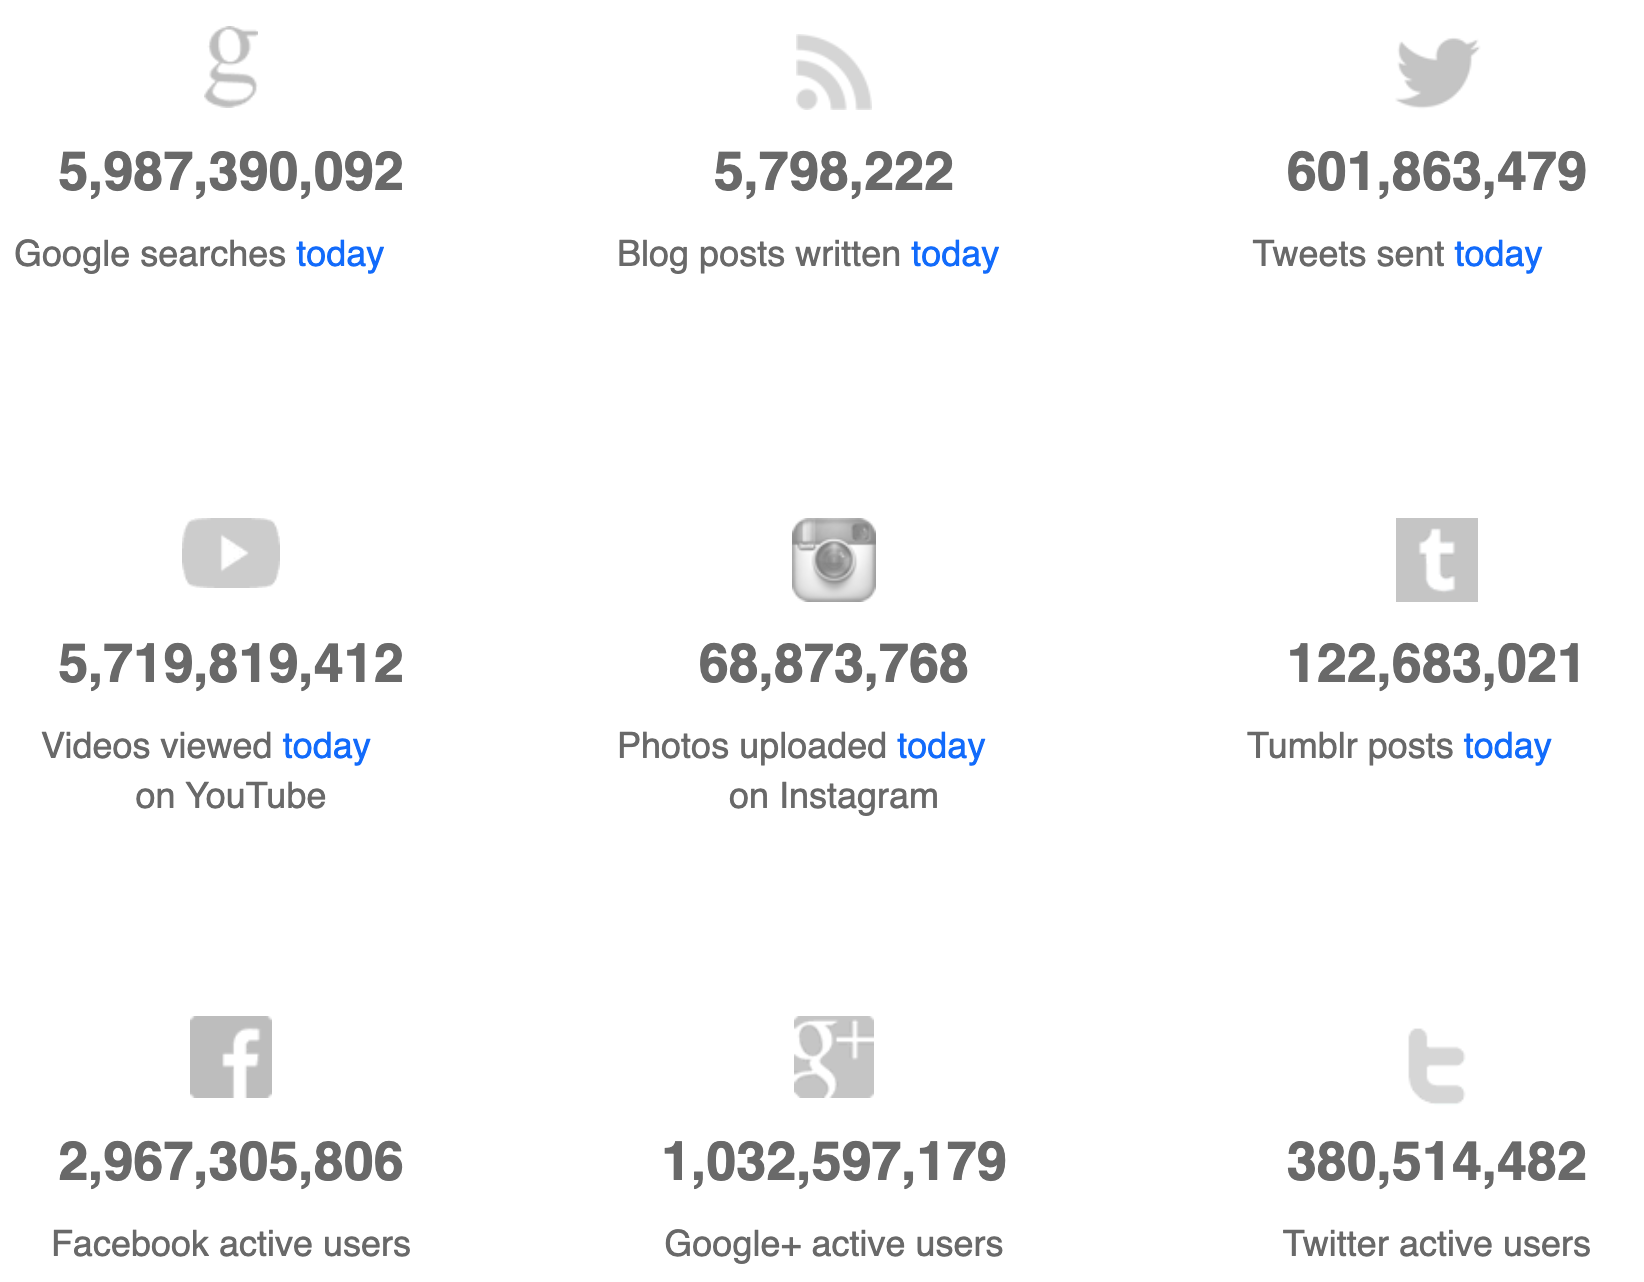
\includegraphics[scale=0.3]{internet_stats.png} \centering
  
  \vfill
  \footnotesize \url{https://www.internetlivestats.com/}
  
  
  \end{frame}
  
  
  %%%%%%%%%%%%%%%%%%%%
  \begin{frame}{Types of Existing Research with Images as Data}
  \large{Causal Framework}
  
  \begin{itemize}
      \item Images as explanatory/independent variable
      \begin{itemize}
          \item Boussalis et al. (APSR 2021): \textit{How candidate emotional expressions in televised debate affect voting preferences?}
          \vspace*{0.2cm}
          \item Casas and Webb Williams (PRQ 2018):\textit{ Which Black Lives Matter images mobilized more supporters?}
      \end{itemize}
      \vspace*{0.5cm}
      \item Images as dependent variable
      \begin{itemize}
          \item Dietrich and Ko (CCR 2022): \textit{TV coverage of Dr. Fauci during the covid pandemic}
          \vspace*{0.2cm}
          \item Michelle Torres (working paper): \textit{How do different news organizations choose different pictures to accompany articles about Black Lives Matter?}
      \end{itemize}
  \end{itemize}
  
  \end{frame}
  
  %%%%%%%%%%%%%%%%%%%%
  \begin{frame}{Types of Existing Research with Images as Data}
  \large{As a Measurement Strategy}
  
  \begin{itemize}
      \setlength\itemsep{0.2cm} 
      \item Images can contain information about electoral incidents and fraud (Callen and Long (2015); Cant\'{u} (2019))
      
      \item Images can help us identify and classify protest events (Zhang and Pan (2018), Won, Steinert-Threlkeld and Joo (2017))
      
      \item Nighttime lights imagery as a proxy for economic development (many authors)
      
      \item Digitized historical maps as evidence of road quality variation (Hunziker et al (working paper))
      
      \item Videos/Images can help us measure cooperation in legislative politics (Dietrich 2020)
  \end{itemize}
  
  \end{frame}
  
  %%%%%%%%%%%%%%%%%%%%
  \begin{frame}{Types of Existing Research with Images as Data}
  \large{Methodological contributions}
  
  \begin{itemize}
  \setlength\itemsep{0.2cm}
      \item Methodological reviews (Webb Williams et al. 2020; Torres \& Cantu 2021)
      
      \item Unsupervised clustering (Zhang \& Peng 2022; Casas et al.(working paper); Torres (working paper))
      
      \item Limitations \& biases (Schwemmer et al. 2020)
      
      \item Extracting/leveraging aesthetic features (Peng 2021)
      
      
  \end{itemize}
  
  \end{frame}
  
  %%%%%%%%%%%%%%%%%%%%
  \begin{frame}{Available Automated Image Analysis Methods}
  \large{Object detection \& recognition}
  
  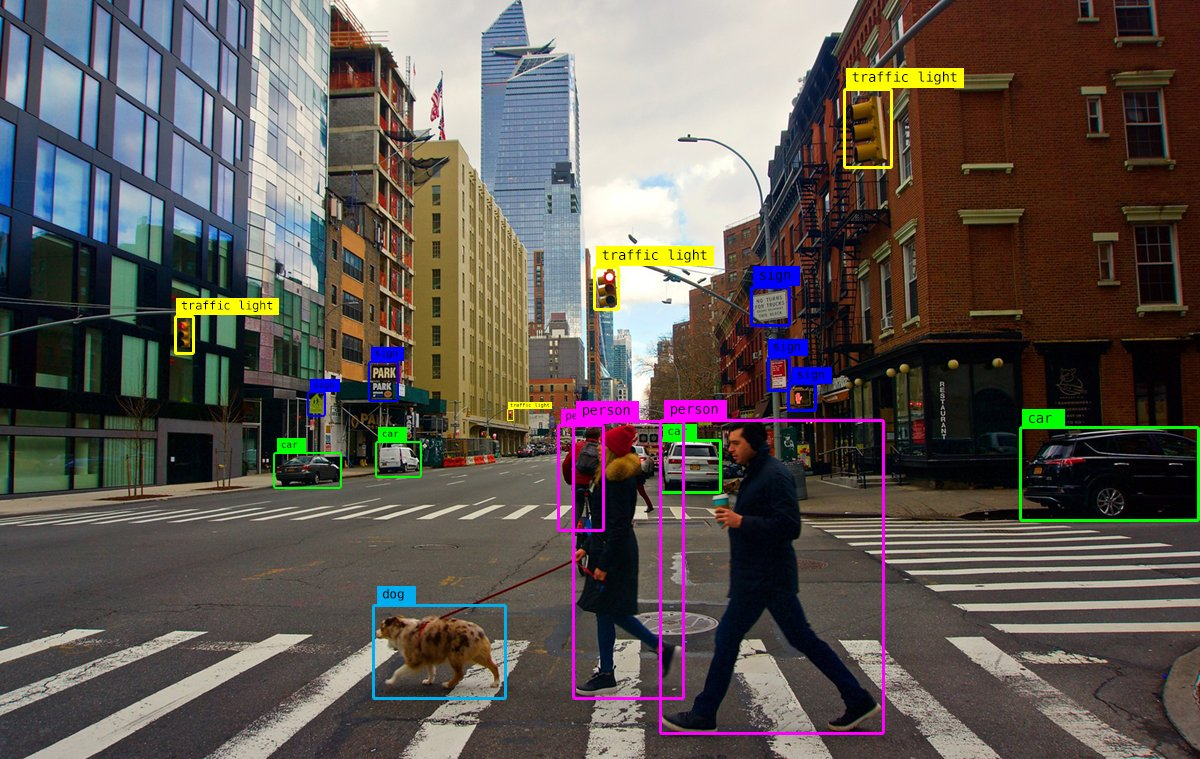
\includegraphics[scale=0.2]{object.jpeg} \centering
  
  \end{frame}
  
  
  %%%%%%%%%%%%%%%%%%%%
  \begin{frame}{Available Automated Image Analysis Methods}
  \large{Face detection \& recognition}
  
  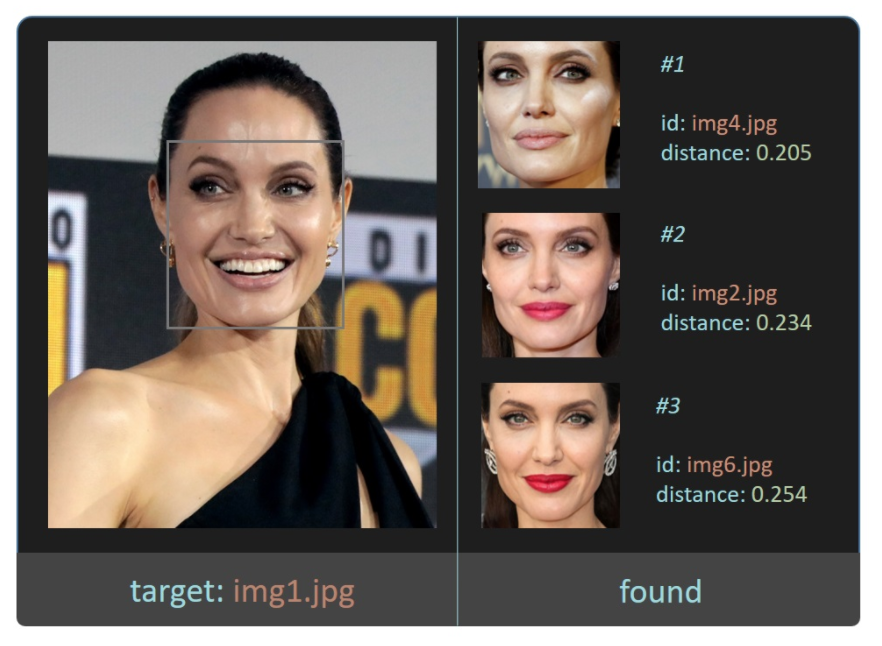
\includegraphics[scale=0.5]{angelina.png} \centering
  
  \end{frame}
  
  %%%%%%%%%%%%%%%%%%%%
  \begin{frame}{Available Automated Image Analysis Methods}
  \large{Face analysis}
  
  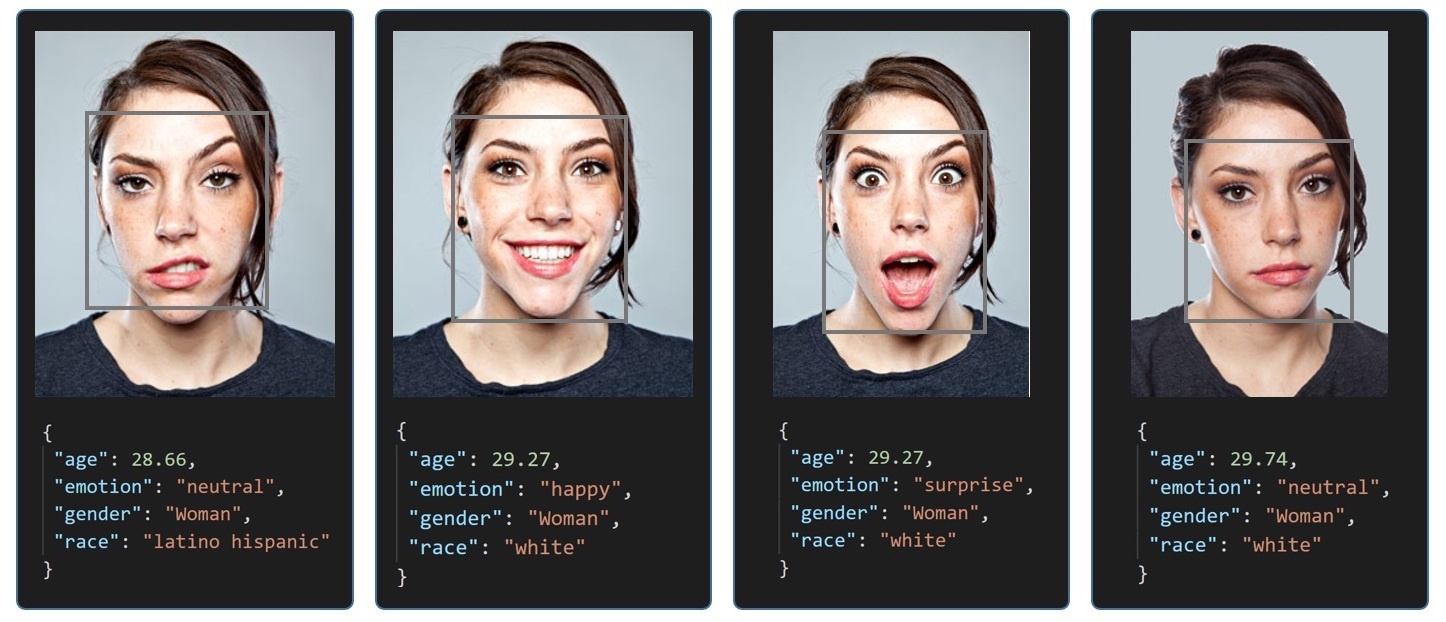
\includegraphics[scale=0.2]{deepface_faceanalysis.jpeg} \centering
  
  \end{frame}
  
  %%%%%%%%%%%%%%%%%%%%
  \begin{frame}{Available Automated Image Analysis Methods}
  \large{Image Similarity}
  
  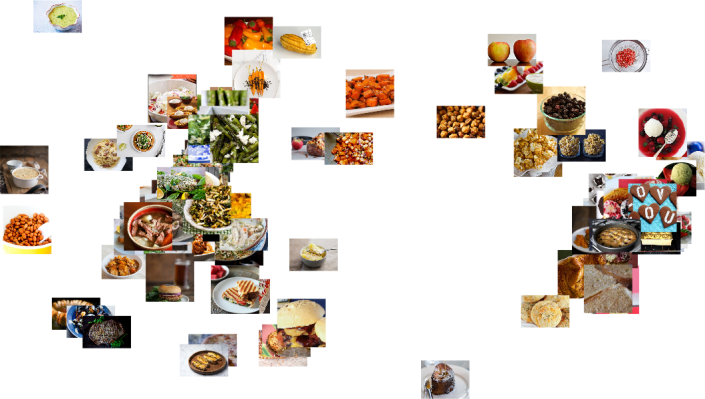
\includegraphics[scale=0.8]{image_similarity.png} \centering
  
  \end{frame}
  
  %%%%%%%%%%%%%%%%%%%%
  \begin{frame}{Available Automated Image Analysis Methods}
  \large{Unsupervised Clustering}
  
  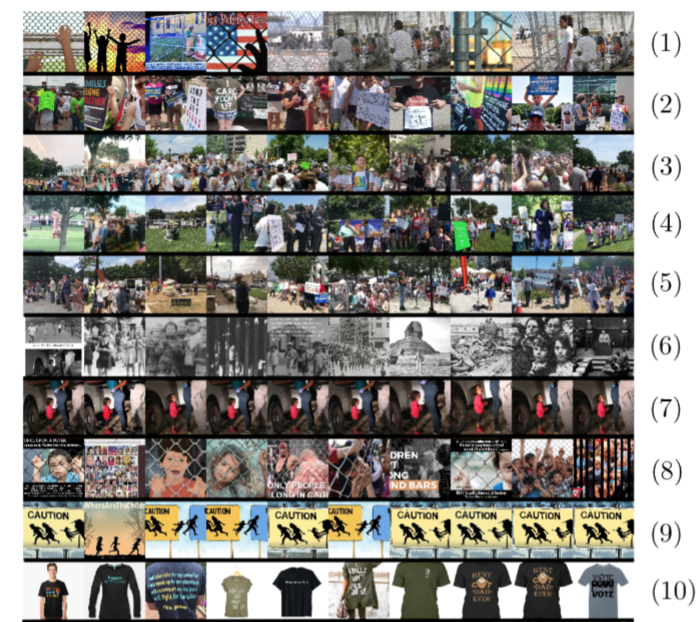
\includegraphics[scale=0.7]{unsupervised_clustering.png} \centering
  
  \end{frame}
  
  %%%%%%%%%%%%%%%%%%%%
  \begin{frame}{Available Automated Image Analysis Methods}
  \large{And many others...}
  
  \begin{itemize}
      \item Text extraction (OCR)
      \item Caption generation
      \item Sentiment analysis (evoked emotions)
      \item Visual aesthetics analysis
      \item etc...
  \end{itemize}
  
  \end{frame}

  

\begin{frame}{More and more in communication science}
  A recent turn towards automated content analysis of visual content -- including a whole special issue on ``images as data'' in CCR \parencite{Casas2022}:
 
  \begin{enumerate}
  \item Images become more important (e.g., Instagram)
  \item More images available to social scientists (not only social media, but also repositories, archives, \ldots)
  \item New computational methods available
  \end{enumerate}
\end{frame}



\begin{frame}{Yet, not as mainstream as compuational textual methods}
``Moreover, [\ldots] there are
starting costs to learning [\ldots]  computer vision
methods, given that the jargon is often very computer-science and machine-
learning specific, and state-of-the-art libraries and packages are available
mostly in Python while social scientists are often more used to working
in the R programming language. Thus
the special issue aims to lower
start-up costs for scholars interested in using images-as-data methods in
their research.''
\parencite[p.~3]{Casas2022}
\end{frame}

\begin{frame}[standout]
And yet, as we'll see, it's not that big a leap from what we already know!
\end{frame}


\begin{frame}{Some examples}
  \begin{block}{\cite{Chen2022}}
    \textbf{Can we detect conspiracy videos?}

    It seems we can, based (also) on visual features like contrast and brightness.

    Techniques: Manual feature extraction + classical ML
  \end{block}
\end{frame}


\begin{frame}{Some examples}
  \begin{block}{\cite{Jurgens2022}}
    \textbf{How are age and gender represented on German TV?}

    There seems to be discrimination against women and elderly

    Techniques: Deep learning using pre-trained models
  \end{block}
\end{frame}



\begin{frame}{Some examples}
  \begin{block}{\cite{Joo2022}}
    \textbf{How do politcians represent themselves visually in the media?}

    It seems there are party and gender differences
    
    Techniques: Commercial API
  \end{block}
\end{frame}


\begin{frame}[standout]
  You can find some more examples here:
  \url{https://computationalcommunication.org/ccr/issue/view/8}
\end{frame}

\begin{frame}{Latest trends}
  \begin{itemize}
  \item moving images (aka videos)
  \item combining text and visuals
  \item really hot: Transformers that model them simultaneously (!!!): ``we present data2vec, a framework that uses the same learning method for either speech, NLP or computer vision. The core idea is to predict latent representations of the full input data'' \parencite{Baevski2022}
  \end{itemize}

\end{frame}



\question{But how do we do all of this? (not data2vec, that's for another time\ldots)}


\subsection{Representing multimedia data}

\begin{frame}{What exactly is an image to a computer?}
  \begin{itemize}
  \item Just a bunch of numbers
  \item Most images are based on the RGB (red-green-blue) model -> remember primary colors?
  \item So every image is a three-dimensional matrix with width x height x depth
  \end{itemize}
\end{frame}

\begin{frame}{What an image looks like}

  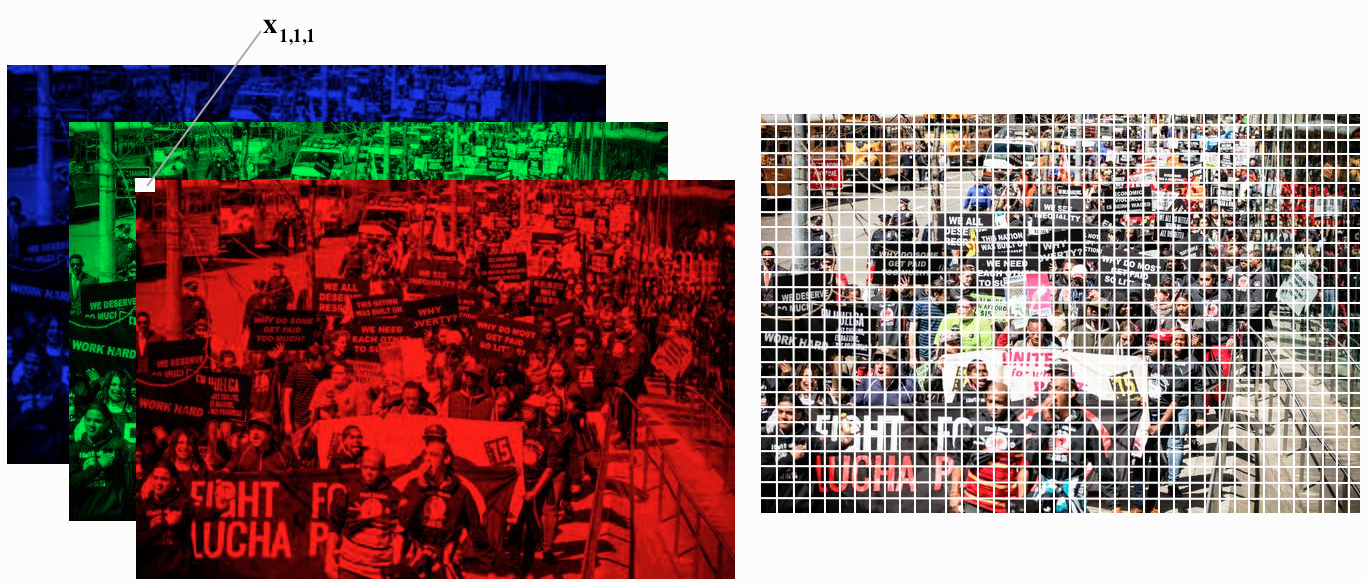
\includegraphics[scale=0.15]{image_rgb.png}
  
  $\mathbf{X} = $ \\ \vspace{0.2cm}
\scriptsize
\color{red}
$
\begin{bmatrix}
x_{111} & x_{112} & \hdots &  x_{11n} \\
x_{121} & x_{122} & \hdots &  x_{12n} \\
x_{131} & x_{132} & \hdots &  x_{13n}  \\
x_{141} & x_{142} & \hdots &  x_{14n}  \\
	\vdots & \vdots \\

x_{1n1} & x_{1n2} & \hdots &  x_{1nn}  
\end{bmatrix}
$ \color{black} \textbf{,} \color{green}
$
\begin{bmatrix}
x_{211} & x_{212} & \hdots &  x_{21n} \\
x_{221} & x_{222} & \hdots &  x_{22n} \\
x_{231} & x_{232} & \hdots &  x_{23n}  \\
x_{241} & x_{242} & \hdots &  x_{24n}  \\
	\vdots & \vdots \\

x_{2n1} & x_{2n2} & \hdots &  x_{2nn}  
\end{bmatrix}
$ \color{black} \textbf{,} \color{blue}
$
\begin{bmatrix}
x_{311} & x_{312} & \hdots &  x_{31n} \\
x_{321} & x_{322} & \hdots &  x_{32n} \\
x_{331} & x_{332} & \hdots &  x_{33n}  \\
x_{341} & x_{342} & \hdots &  x_{34n}  \\
	\vdots & \vdots \\

x_{3n1} & x_{3n2} & \hdots &  x_{3nn}  
\end{bmatrix}
$
\end{frame}

\begin{frame}{Amount of pixels}
  \begin{itemize}
    \item A Grayscale image only has one layer, so for a $200\times 300$ image, we have a two-dimensional matrix with $200\times 300 = 60,000$ pixels
    \item The same size image in color is: $200\times 300\times 3 = 180,000$ integers between 0 and 255
  \end{itemize}
\end{frame}

\begin{frame}{What can we do with images in Python?}
  \begin{itemize}
  \item PIL (Pillow), the Python Image Library, provides many typical image operations (reading, displaying, cropping, color transformations)
  \item That's cool for batch processing (a for-loop and you can resize thousands of images\ldots)
  \item But more imporantly: \textbf{It's just a vector/matrix of integers, so we can do machine learning just like we did before!}
  \end{itemize}
\end{frame}

  

\subsection{Classic SML}

\begin{frame}{First approach}
  \begin{itemize}
  \item If each picture is just a vector of integers, scikit-learn works \emph{exactly the same} as for survey data (Chapter 8) or text (Chapter 11).
  \item Typical example: recognizing hand-written characters with a Random Forest (Example 14.10) or a Support Vector Machine\footnote{\url{https://scikit-learn.org/stable/auto\_examples/classification/plot\_digits\_classification.html}}
  \end{itemize}
\end{frame}


\begin{frame}[fragile]{This is impressive!}
\begin{lstlistingoutputtiny}
Classification report for classifier SVC(gamma=0.001):
              precision    recall  f1-score   support

           0       1.00      0.99      0.99        88
           1       0.99      0.97      0.98        91
           2       0.99      0.99      0.99        86
           3       0.98      0.87      0.92        91
           4       0.99      0.96      0.97        92
           5       0.95      0.97      0.96        91
           6       0.99      0.99      0.99        91
           7       0.96      0.99      0.97        89
           8       0.94      1.00      0.97        88
           9       0.93      0.98      0.95        92

    accuracy                           0.97       899
   macro avg       0.97      0.97      0.97       899
weighted avg       0.97      0.97      0.97       899
\end{lstlistingoutputtiny}
\tiny{\url{https://scikit-learn.org/stable/auto\_examples/classification/plot\_digits\_classification.html}}

\end{frame}


\question{Can you explain why this works?}


\begin{frame}{The intuition behind it}
  If the images are cropped and resized equally (!)\ldots

  \vspace{1cm}
  
  \ldots then the pixels in the center should be white for a 0 but dark for a 8.
\end{frame}


\question{Can you name tasks for which you think this would \emph{not} work?}




\subsection{Deep Learning}

\question{Do you remember what the reason for using deep learning in text classification was?}

\begin{frame}{Say we want to recognize whether an image is a cat or a dog\ldots}
  \begin{itemize}
  \item Can we really say that the color of a pixel maps directly to the ``catness'' or ``dogness'' of the picture?
  \item Or should it not rather be about their fur, the shape of the ears, \ldots
  \item But it seems impossible to engineer these features by hand :-(
  \end{itemize}

  \pause

  Let's use a deep neural network to learn them!
\end{frame}


\begin{frame}{How do we do this?}
  \begin{itemize}
  \item For deep learning, we use \texttt{keras} instead of \texttt{scikit-learn}
  \item You need to specify the \emph{architecture} of the network
  \item The process is resource-intensive
  \end{itemize}
\end{frame}


\begin{frame}{Working with images}
  There are many frameworks, but particularly interesting for us:
  \begin{itemize}
  \item The Convolutional Neural Network (CNN): A neural network in which the layers are not fully connected
  \item We have talked about this before, remember?
  \end{itemize}
\end{frame}

\begin{frame}{Convolutional Neural Nets for Computer Vision}
  \noindent Convolutional layers: weights (\textbf{filters}) are not connected to the whole \textbf{input volume}: convolution.\\ \footnotesize Click \href{http://cs231n.github.io/convolutional-networks/}{\underline{here}} for a full visualization by the Stanford cs231 folks.
  
  \begin{center}
  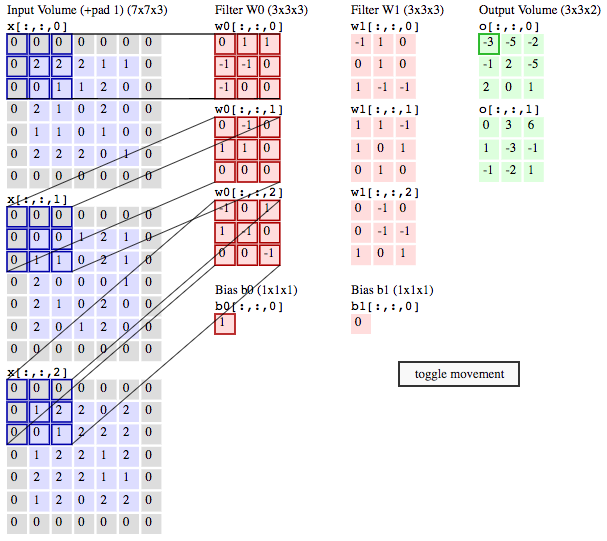
\includegraphics[scale=0.3]{05-convolution-example.png} 
  \end{center}
  
  
  \end{frame}

  \begin{frame}{Some terminology}
    \begin{itemize}[<+->]
      \setlength\itemsep{0.2cm}
      \item \textbf{input volume}: a 3-dimensional input
      \item \textbf{convolutional layer}: a 4-dimensional parameter layer where convolutional filters are applied to the input volume; of size FxFxNxK where F is the width and height of the filter, N is the number of filter dimensions, and K is the number of filters $\rightarrow$ 3x3x3x2 in the previous example
      \item \textbf{stride}: the number of pixels we move the filter at a time. This is 2 in the previous example
      \item \textbf{zero-padding}: adding zeros around the input border (often done to avoid deforming input images)
      \item \textbf{pooling layer}: a layer where we reduce the size the output of a convolutional layer. From 224x224x3x64 to 112x112x3x64 for example.
      \end{itemize}
  \end{frame}


  \begin{frame}{...and more terminology}
    \begin{itemize}
      \item \textbf{fully connected layer}: a layer of weights that is connected to the whole input volume. These are usually at the end of a network.
      \item \textbf{softmax}: a multi-class classifier. This is basically a multinomial logit model that uses the output of the last fully-connected layer to predict the final classes of interest
      \end{itemize}
  \end{frame}

  \begin{frame}{Convolutional Neural Nets for Computer Vision}
    \large{This is how a ConvNet looks like} \vspace{0.1cm}
    \begin{center}
    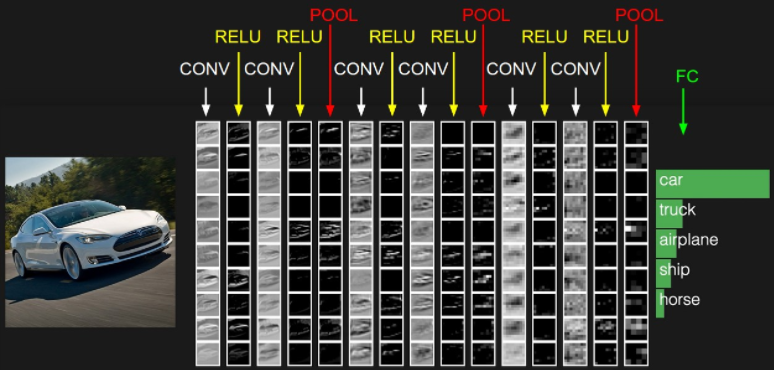
\includegraphics[scale=0.4]{06-convnet-example.png} 
    \end{center}
    \end{frame}

\begin{frame}{Training your own neural network?}
  If you have a very specific task and an annotated dataset -- sure!

  But:
  \begin{itemize}
  \item Can be \emph{very} resource-intensive
  \item Often, very large amounts of training data needed
  \item There are so many architectures, and you can't possibly know the best ones without being an expert
  \end{itemize}
\end{frame}

\begin{frame}{Training your own neural network?}
  \begin{block}{Solution 1: Using a pre-trained model}
Just use a CNN that already is trained (Examples 14.14--14.17). Make sure to read up on the specific model you are using.
  \end{block}
\end{frame}

\begin{frame}{Training your own neural network?}
  \begin{block}{Solution 2: Fine-tuning a pre-trained model}
If you have a labeled dataset, you can start with an existing pre-trained model and then fine-tune it with your data (many tutorials online)
  \end{block}

  There is also a really, really cool approach called CLIP that uses transformers to embed images and texts in the same  (!) vector space \parencite{radford2021clip} -- \tiny{\url{https://huggingface.co/docs/transformers/model_doc/clip}}

\end{frame}


\begin{frame}{Training your own neural network?}
  \begin{block}{Solution 3: A (commercial) API}
    (next section)
  \end{block}
\end{frame}

\subsection{(Commercial) APIs}

\begin{frame}{What is it?}
  \begin{itemize}
  \item You send an image to the API and get a set of labels back
  \item Under the hood: pre-trained neural networks
  \item Very much black box: you have no idea where the labels come from
  \item Prominent players: Clarifai, Google Cloud Vision, Microsoft
  \item Usually paid but often free for small projects and/or academic use
  \end{itemize}

\end{frame}


\begin{frame}{Automated Visual Content Analysis  \parencite{Araujo2020b}}
  \begin{alertblock}{Problem}
The labels do not correspond what one may be theoretically interested in.
  \end{alertblock}

  \pause
  
\begin{block}{Solution}
  \begin{itemize}
  \item Annotate a set of images manually using a codebook
  \item Use the labels provided by the API as features to train a classifier to predict the annotations
  \item Thus, we essentially have transformed the image prediction task to a textual prediction task
  \end{itemize}
\end{block}
\end{frame}



\begin{frame}{Is it difficult to use a computer vision API?}
  \textbf{No.}

All providers provide Python code examples, e.g. \url{https://cloud.google.com/vision/docs/detect-labels-image-client-libraries}
  
\end{frame}

\begin{frame}{Biases: Garbage in, garbage out}
  
  \begin{itemize}[<+->]
      \setlength\itemsep{0.2cm}
      \item Known issues: Gender and Race
      \item Joy Buolamwini (MIT) \textrightarrow{} Gender Shades
      \item Fairness, Accountability, and Transparency conference
      \item Best option: Knowing the training data, proper validation
      \item Schwemmer et al (2020) show an example on how to detect biases in commercial models
  \end{itemize}
  \vspace*{0.4cm}
  
  
\includegraphics[scale=0.2]{gender_race.png} \centering
  
  \end{frame}
  
  \begin{frame}{A recent example}
  
\includegraphics[scale=0.3]{dutch_case_bias.png} \centering
  \end{frame}

  \begin{frame}{Privacy: My face is on that picture}
    
    \begin{itemize}[<+->]
        \setlength\itemsep{0.2cm}
        \item GDPR: Private data needs to be anonymized
        \item Especially important when working with social media images
        \item Common strategies: Pixellation \& Blurring (not bulletproof!)
        \item Sharing of data? Using external services for data? \textrightarrow{} Consider using open-source taggers run locally 
    \end{itemize}
    \vspace*{0.25cm}
    
    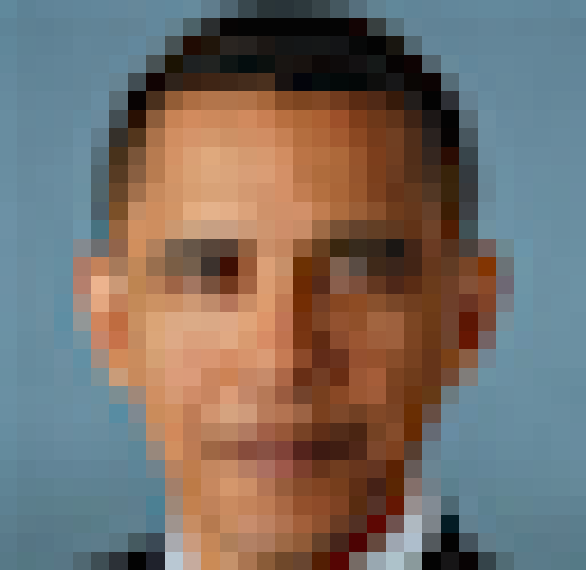
\includegraphics[scale=0.2]{pixel-barack.png} \centering
    
    \end{frame}

    \begin{frame}{Privacy: My face is on that picture}
      
      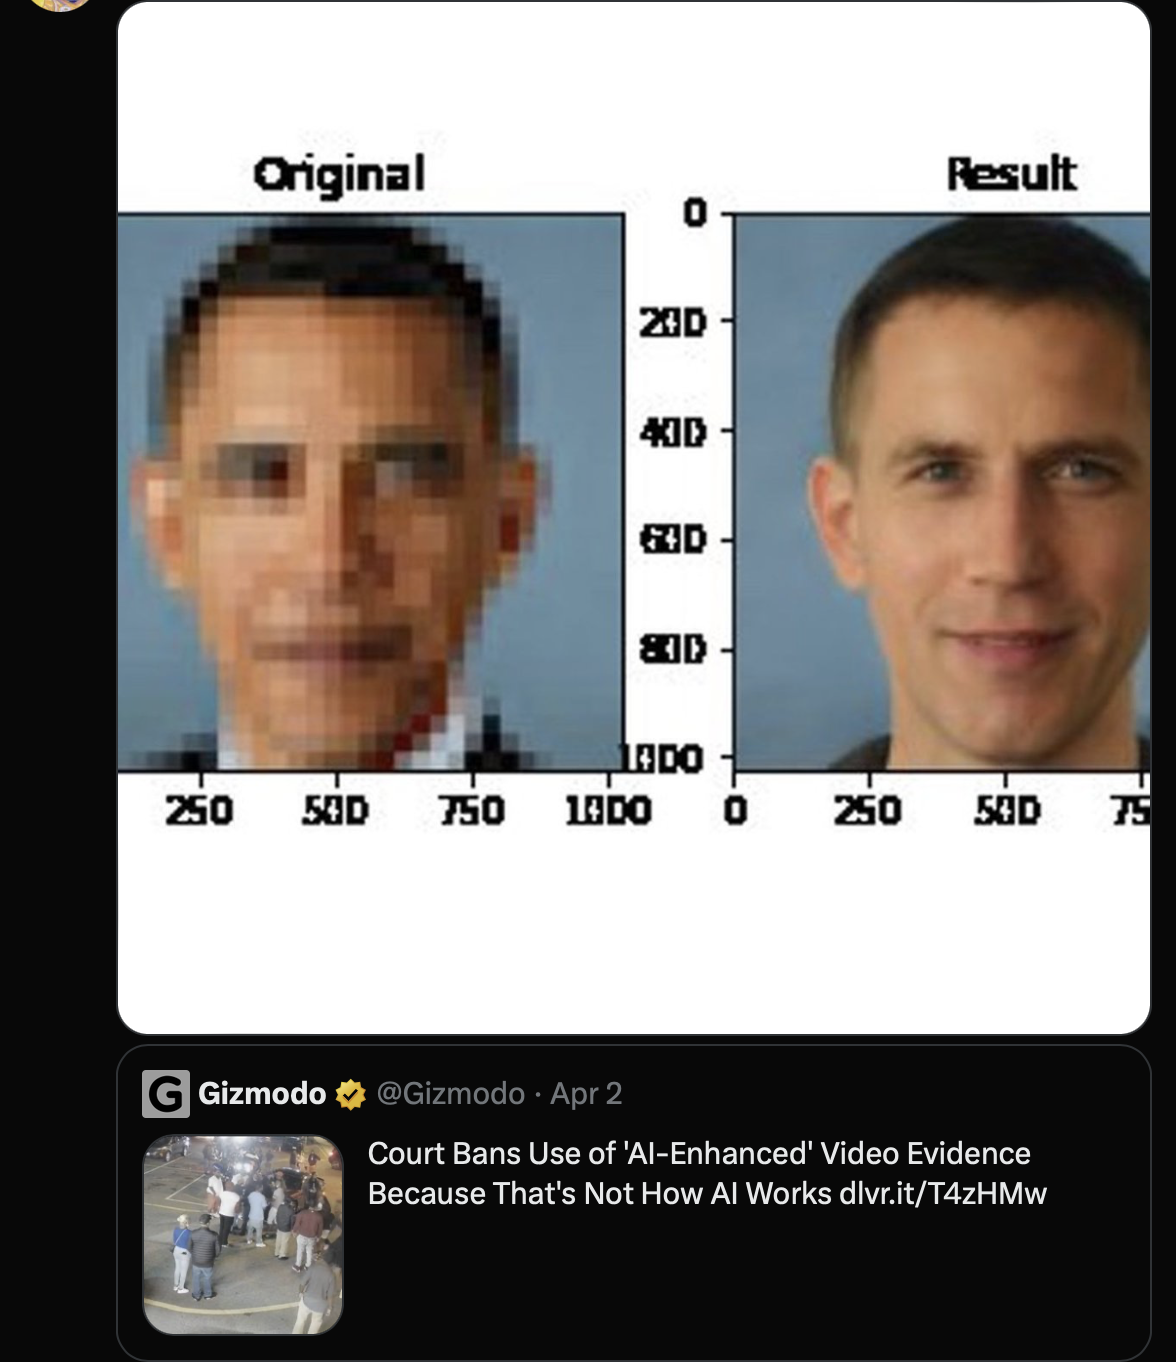
\includegraphics[scale=0.2]{barack_twitter.png} \centering
      
      \end{frame}
  


\begin{frame}{Further reading}
  \begin{itemize}
  \item all the articles in the special issue edited by \cite{Casas2022}
  \item a short book by \cite{Webbwilliams2020}
  \item the study by \cite{Araujo2020b}
  \item This medium post on CNNs:  \url{https://towardsdatascience.com/convolutional-neural-networks-explained-9cc5188c4939}
    \end{itemize}
\end{frame}



\begin{frame}{Final remark}
  The black box nature of (most of) these techniques \emph{is} a big problem from a social-science and epistemological point of view: in particular, known and un-known biases!

As always, but maybe especially here: Never take the outcome as a given -- it needs interpretation and critical reflection!

\end{frame}




\section{Next steps}
\begin{frame}[standout]
Let's have a look together at the course manual regarding the final project.
\end{frame}

\begin{frame}{Examples}
On Canvas under ``modules'', you find some example projects. Note that these are not necessarily \emph{perfect} assignments, and also that the content of the course (and hence, expectations) are not be fully identical to the years in which a specific assignment was made. \textbf{In particular, there may be more advanced and more appropriate techniques available now!}
\end{frame}

\begin{frame}{Friday}
On Friday, you can \emph{either} work on one of the computer vision examples discussed today and/or in the book.

\emph{Or} you start working on your final project.

\end{frame}


\begin{frame}[allowframebreaks,plain]
\printbibliography
\end{frame}



\end{document}
